
\documentclass[11pt,a4paper]{article}
\usepackage[margin=25mm]{geometry}
\usepackage{graphicx}
\usepackage{booktabs}
\usepackage{array}
\usepackage{hyperref}
\usepackage{xurl}
\usepackage{float}
\usepackage{xcolor}
\usepackage{enumitem}
\hypersetup{colorlinks=true, linkcolor=blue, urlcolor=blue, citecolor=blue}
\setlist[itemize]{leftmargin=1.2em}
\title{Claim-Bounded Threshold, Hysteresis, and Rescue-Regime Audits for a Sleep-Like Recovery-Transition Toy Network\\\large DTTS v0.3.0 Synthesis Addendum}
\author{Keiji Yoshimura\\Independent Researcher}
\date{2026}
\begin{document}
\maketitle

\noindent\textbf{Repository:} \url{https://github.com/yokken0907/dynamical-threshold-theory-of-sleep}

\medskip

\begin{abstract}
This addendum summarizes DTTS v0.2.0--v0.2.8 toy-model audits for sleep-like recovery transitions in finite adaptive networks. The supported claim is intentionally narrow: within the implemented network-dynamical toy-model sequence, threshold-like sleep-gate onset, hysteresis-like persistence, structurally aligned selective protection, perturbation-recovery response, topology/noise robustness, failure boundaries, and rescue-sensitive regimes were observed under tested settings. Frozen minimal rescue policies generalized across holdout seeds, simplified topologies, and noise levels for most rescue-sensitive regimes, while weak-protection conditions remained unstable under harsher holdout. This is not a clinical sleep model, biological sleep validation, EEG or wearable-device predictor, diagnostic method, treatment tool, or complete biological theory of sleep.
\end{abstract}

\section{Reader guidance and claim boundary}
The Dynamical Threshold Theory of Sleep (DTTS) is treated here as a reduced mathematical prototype for sleep-like recovery transitions in adaptive finite networks. The addendum does not assert that the model explains human sleep, animal sleep, neurological sleep regulation, sleep disorders, EEG signatures, or clinical outcomes. Its role is methodological: to test whether a specified toy network can display threshold-like recovery-gate dynamics, selective protection, failure regimes, and frozen rescue-policy generalization.

Allowed statements are limited to the implemented toy-model sequence and its generated evidence archive. Forbidden statements include clinical sleep diagnosis, medical advice, treatment guidance, human or animal sleep-data validation, EEG or wearable-device prediction, and a complete biological theory of sleep.

\section{Audit sequence}
The v0.2.x sequence was designed to move from constructive positive tests to negative controls, robustness checks, failure-boundary exploration, mechanism-rescue classification, and frozen holdout. Table~\ref{tab:ledger} summarizes the locked phase ledger.

\begin{table}[H]
\centering
\small
\begin{tabular}{p{0.12\linewidth}p{0.32\linewidth}p{0.46\linewidth}}
\toprule
Phase & Role & Locked contribution \\
\midrule
v0.2.0 & Threshold/protection preflight & Threshold-drive candidate identified; sleep-like gate onset and protection controls established. \\
v0.2.1 & Closed-loop hysteresis & Baseline hysteresis-like gap exceeded memoryless control. \\
v0.2.2 & Circadian/multi-cycle audit & Circadian-like permissive gate modulated onset timing; protection remained active. \\
v0.2.3.1 & Perturbation recovery & Acute load pulses evoked gate response; no-gate control suppressed it. \\
v0.2.4 & Topology/noise robustness & Core gate/protection effects persisted across simplified topology and noise settings. \\
v0.2.5 & Conservative envelope & No failure boundary found inside the conservative envelope; claims restricted to that envelope. \\
v0.2.6 & Expanded failure boundary & Failure cases identified; DTTS behavior shown not to be universal. \\
v0.2.7 & Mechanism rescue & Failure modes separated into gate, protection, and unresolved-load boundaries with distinct rescue responses. \\
v0.2.8 & Frozen rescue holdout & Frozen rescue policies generalized for most rescue-sensitive regimes; weak-protection remained unstable. \\
\bottomrule
\end{tabular}
\caption{Claim-bounded DTTS v0.2.0--v0.2.8 phase ledger.}
\label{tab:ledger}
\end{table}

\section{Synthesis result}
The locked synthesis claim is:

\begin{quote}
Within the implemented finite adaptive-network toy-model sequence, DTTS-like sleep-gate onset, hysteresis-like persistence, structurally aligned selective protection, perturbation-recovery response, and topology/noise robustness were observed within tested regimes. Expanded audits identified failure boundaries, and frozen minimal rescue policies generalized across holdout seeds, simplified topologies, and noise levels for most rescue-sensitive regimes, while weak-protection conditions remained unstable under harsher holdout. This is a claim-bounded network-dynamical toy-model result, not a biological or clinical sleep claim.
\end{quote}

The most important negative result is that DTTS-like behavior is not universal. Low drive, high threshold, weak gate gain, weak protection, and unresolved-load regimes can weaken or disrupt the desired signatures. This converts the theory from a broad sleep claim into a bounded regime-classification framework.

\section{Frozen rescue holdout}
The v0.2.8 frozen-rescue holdout used six scenario classes, five simplified topologies, and four noise levels, yielding 240 holdout cells. The mean frozen-policy pass rate was 0.7729. Native pass count was 1; rescue holdout pass count was 4; unstable rescue boundary count was 1; persistent failure boundary count was 0. The remaining unstable boundary was weak protection, indicating that structural protection is not merely decorative but a central condition for the modeled selective renormalization effect.

\begin{figure}[H]
\centering
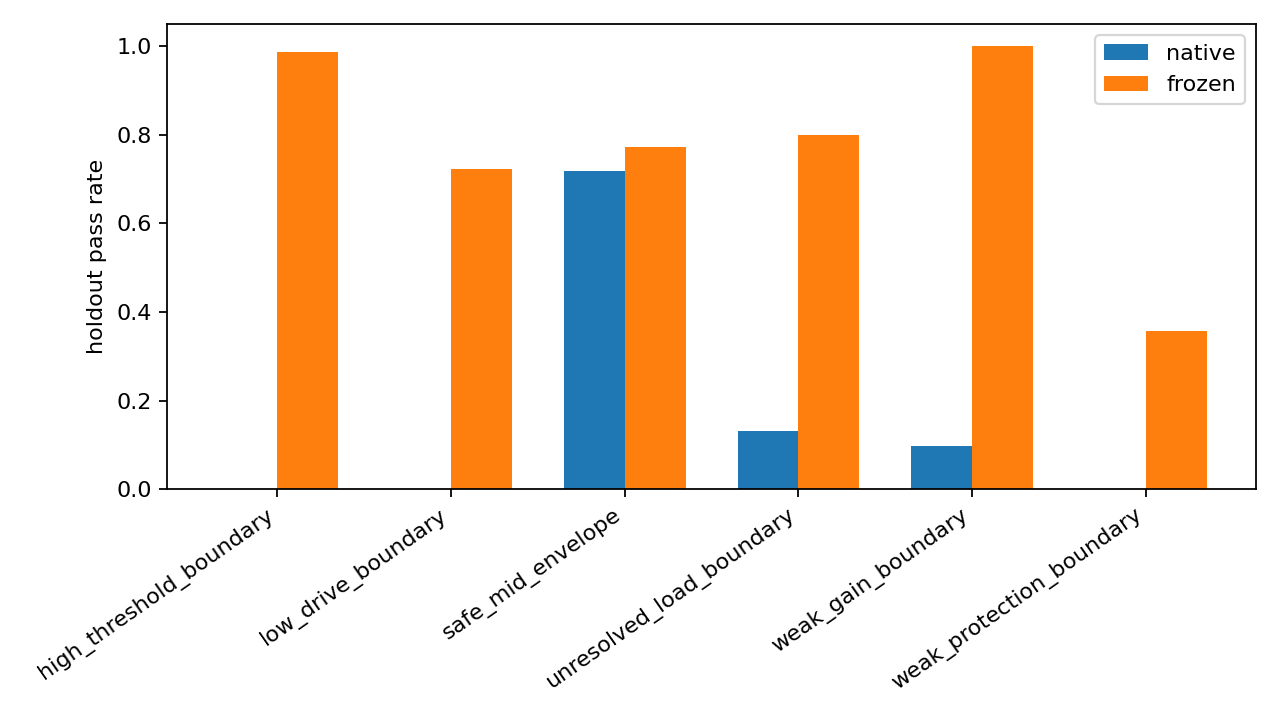
\includegraphics[width=0.96\linewidth]{dtts_v028_frozen_vs_native_pass_rates.png}
\caption{Frozen rescue-policy pass-rate comparison from the v0.2.8 holdout audit.}
\label{fig:frozen-pass}
\end{figure}

\begin{figure}[H]
\centering
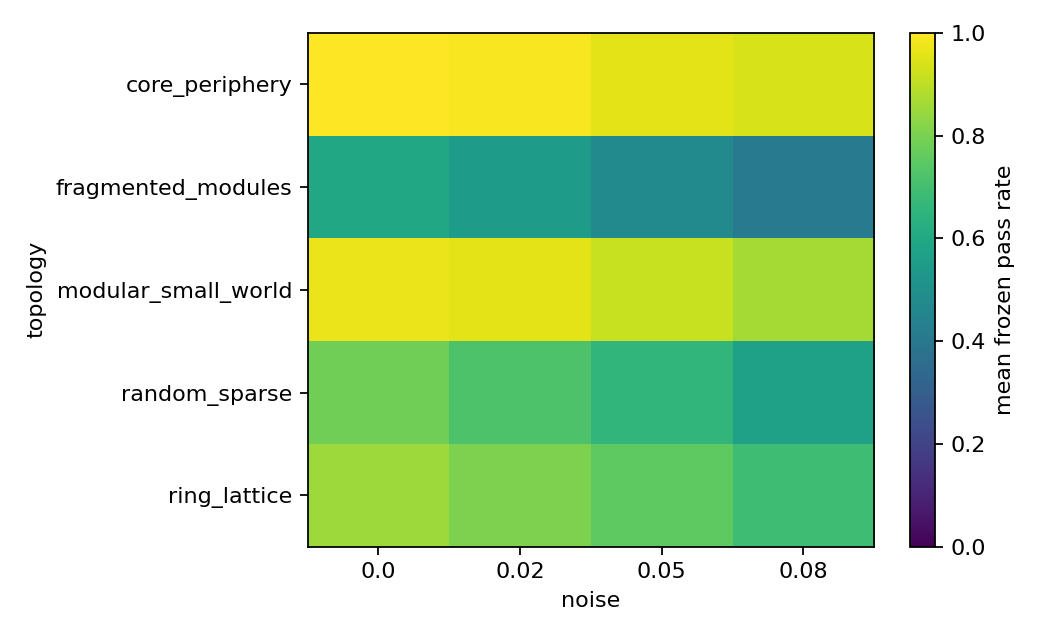
\includegraphics[width=0.90\linewidth]{dtts_v028_topology_noise_holdout_heatmap.png}
\caption{Topology/noise holdout heatmap for frozen rescue-policy generalization.}
\label{fig:heatmap}
\end{figure}

\section{Interpretation}
The addendum supports a restrained interpretation: the DTTS mechanism can be organized as a network-dynamical recovery-transition prototype with four interacting elements: load accumulation, thresholded gate onset, structurally aligned selective protection, and regime-dependent rescue sensitivity. The model is useful as a hypothesis-generating diagnostic scaffold for reduced network dynamics. It is not a validated account of biological sleep.

\section{Limitations}
The audits use simplified networks, synthetic load dynamics, synthetic protection fields, and internal toy-model controls. No human data, animal data, polysomnography, EEG, wearable-device data, clinical sleep annotation, pharmacological intervention, or treatment outcome is included. The phrase ``sleep-like'' refers only to a modeled recovery-gate transition, not to physiological sleep.

\section{Evidence and reproducibility}
The supporting evidence archive contains the v0.3.0 synthesis report, claim lock, phase ledger, next-step note, selected figures, and the uploaded v0.2.0--v0.2.8 output-derived synthesis. The public GitHub repository is available at \url{https://github.com/yokken0907/dynamical-threshold-theory-of-sleep}. The repository license remains the source-defined Evaluation-Only notice included in the repository root. Zenodo identifiers associated with repository releases should be treated as repository-archive DOIs, not as standalone peer-reviewed article DOIs.

\section*{AI assistance disclosure}
This manuscript and its accompanying repository materials were prepared with AI assistance under the author's direction. The author remains responsible for the final wording, claim boundary, and release decisions.

\section*{References}
\begin{enumerate}
\item Yoshimura, K. \textit{Dynamical Threshold Theory of Sleep: A Network Prototype for Recovery Phase Transitions}. Independent manuscript and repository companion archive, 2026. Repository: \url{https://github.com/yokken0907/dynamical-threshold-theory-of-sleep}. Repository archive DOI history: \href{https://doi.org/10.5281/zenodo.20201448}{10.5281/zenodo.20201448}.
\item DTTS v0.3.0 evidence archive included in this repository release: \texttt{evidence/v030\_synthesis\_outputs/}.
\end{enumerate}

\end{document}
